\documentclass[12pt,a4paper]{article}
\usepackage{algorithm, algpseudocode, amsmath, amssymb, amsthm, bm, csquotes, emf, empheq, geometry, graphicx, hyperref, listings, mhchem, multirow, siunitx, caption, float, longtable}
\usepackage[italicdiff]{physics}
\usepackage[section]{placeins}
\usepackage[justification=centering]{caption}
\usepackage[column=O]{cellspace}
% \usepackage[extrafootnotefeatures]{xepersian}
\hypersetup{colorlinks=true, urlcolor=cyan}

\title{Logistic map and finding Feigenbaum constants}
\author{Zahra Akbari}
\date{}


% \settextfont{}
\linespread{1.2}

\setlength\cellspacetoplimit{5pt}
\setlength\cellspacebottomlimit{3pt}
\newcommand{\multlinecell}[1]{\begin{tabular}[c]{@{}c@{}}#1\end{tabular}}

\newcommand{\qfrac}[2]{\left(\frac{#1}{#2}\right)}
\newcommand{\fsqrt}[2]{\sqrt{\frac{#1}{#2}}}
\newcommand{\ddfrac}[2]{{\displaystyle\frac{\displaystyle #1}{\displaystyle #2}}}
\newcommand{\pdvc}[3]{\qfrac{\partial #1}{\partial #2}_{#3}}
\newcommand{\dbar}{{d\mkern-7mu\mathchar'26\mkern-2mu}}
\newcommand*{\defeq}{\mathrel{\vcenter{\baselineskip0.5ex \lineskiplimit0pt
			\hbox{\scriptsize.}\hbox{\scriptsize.}}}
	=}

\begin{document}
	\maketitle
	\section*{Theory }
	The logistic map is a polynomial mapping (equivalently, recurrence relation) of degree 2, often referred to as an archetypal example of how complex, chaotic behaviour can arise from very simple nonlinear dynamical equations
	\begin{align*}
	x_n &= r x_n (1-x_{n-1}) 
	\end{align*}


	The map is implemented in a julia function with r and $x_n$ argument passing the array consisting the $x_n$. The Initval specifies a random set of 100 initial values.


	
% \pagebreak


	\section*{Plotting}
	The r value goes from 0.001 to 1 (1000 iterations). The computation is repeated for 1000 runs. finally $x_n$ is plotted over r.

			
			\begin{figure}[H]
				\centering
				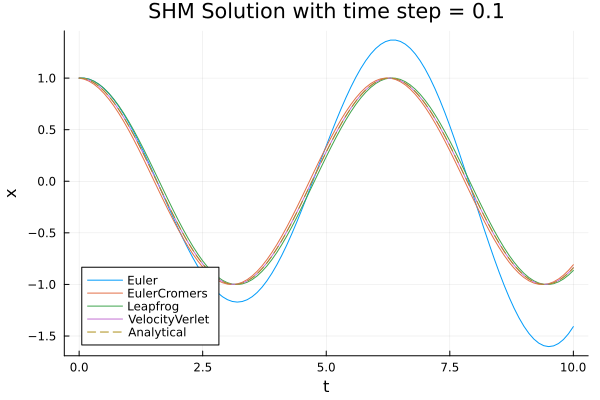
\includegraphics[width=10cm]{graph.png}
				\caption{logistic map with 1000 iterations. }
			\end{figure}

			

	\section{Finding Feigenbaum constans}		
			For finding bifurcation points, we need to check for the points in our graph where the number of points are powers of 2. For doing so, points with a too small distance need to be unified(repetitive points appear becuase of the noise involved.)
			Feigenbaum constans are finally calculated using the bifurcation points.
			Bifurcation points are:\\
			\begin{center}
				
				\begin{tabular}{|c|c|c|c|c|c|}
				\hline
				Branches &2&4&8&16&32 \\
				\hline
				r &0.249& 0.746& 0.864& 0.887& 0.892 \\
				\hline
	
				\end{tabular}

			\end{center}
			

			According to wikipedia, The first Feigenbaum constant is  the limiting ratio of each bifurcation interval to the next between every period doubling:
			\begin{align*}
				\delta &= 4.60
			\end{align*}
			The second Feigenbaum constant is is the ratio between the width of a tine and the width of one of its two subtines (except the tine closest to the fold):
			\begin{align}
				\alpha &= 2.78
			\end{align}
			
			\end{document}
